\documentclass[8pt]{beamer}

% Beamer style
%\usetheme[secheader]{Madrid}
% \usetheme{CambridgeUS}
\useoutertheme{infolines}
\usecolortheme[rgb={0.65,0.15,0.25}]{structure}
% \usefonttheme[onlymath]{serif}
\beamertemplatenavigationsymbolsempty
%\AtBeginSubsection

% Packages
%\usepackage[french]{babel}
\usepackage[latin1]{inputenc}
\usepackage{color}
\usepackage{xspace}
\usepackage{dsfont, stmaryrd}
\usepackage{amsmath, amsfonts, amssymb, stmaryrd}
\usepackage{epsfig}
\usepackage{tikz}
\usepackage{url}
% \usepackage{ulem}
\usepackage{/home/robin/LATEX/Biblio/astats}
%\usepackage[all]{xy}
\usepackage{graphicx}
\usepackage{xspace}
\usepackage{pifont}
\usepackage{marvosym}

% Maths
% \newtheorem{theorem}{Theorem}
% \newtheorem{definition}{Definition}
\newtheorem{proposition}{Proposition}
% \newtheorem{assumption}{Assumption}
% \newtheorem{algorithm}{Algorithm}
% \newtheorem{lemma}{Lemma}
% \newtheorem{remark}{Remark}
% \newtheorem{exercise}{Exercise}
% \newcommand{\propname}{Prop.}
% \newcommand{\proof}{\noindent{\sl Proof:}\quad}
% \newcommand{\eproof}{$\blacksquare$}

% \setcounter{secnumdepth}{3}
% \setcounter{tocdepth}{3}
\newcommand{\pref}[1]{\ref{#1} p.\pageref{#1}}
\newcommand{\qref}[1]{\eqref{#1} p.\pageref{#1}}

% Colors : http://latexcolor.com/
\definecolor{darkred}{rgb}{0.65,0.15,0.25}
\definecolor{darkgreen}{rgb}{0,0.4,0}
\definecolor{darkred}{rgb}{0.65,0.15,0.25}
\definecolor{amethyst}{rgb}{0.6, 0.4, 0.8}
\definecolor{asparagus}{rgb}{0.53, 0.66, 0.42}
\definecolor{applegreen}{rgb}{0.55, 0.71, 0.0}
\definecolor{awesome}{rgb}{1.0, 0.13, 0.32}
\definecolor{blue-green}{rgb}{0.0, 0.87, 0.87}
\definecolor{red-ggplot}{rgb}{0.52, 0.25, 0.23}
\definecolor{green-ggplot}{rgb}{0.42, 0.58, 0.00}
\definecolor{purple-ggplot}{rgb}{0.34, 0.21, 0.44}
\definecolor{blue-ggplot}{rgb}{0.00, 0.49, 0.51}

% Commands
\newcommand{\backupbegin}{
   \newcounter{finalframe}
   \setcounter{finalframe}{\value{framenumber}}
}
\newcommand{\backupend}{
   \setcounter{framenumber}{\value{finalframe}}
}
\newcommand{\emphase}[1]{\textcolor{darkred}{#1}}
\newcommand{\comment}[1]{\textcolor{gray}{#1}}
\newcommand{\paragraph}[1]{\textcolor{darkred}{#1}}
\newcommand{\refer}[1]{{\small{\textcolor{gray}{{\cite{#1}}}}}}
\newcommand{\Refer}[1]{{\small{\textcolor{gray}{{[#1]}}}}}
\newcommand{\goto}[1]{{\small{\textcolor{blue}{[\#\ref{#1}]}}}}
\renewcommand{\newblock}{}

\newcommand{\tabequation}[1]{{\medskip \centerline{#1} \medskip}}
% \renewcommand{\binom}[2]{{\left(\begin{array}{c} #1 \\ #2 \end{array}\right)}}

% Variables 
\newcommand{\Abf}{{\bf A}}
\newcommand{\Beta}{\text{B}}
\newcommand{\Bcal}{\mathcal{B}}
\newcommand{\Bias}{\xspace\mathbb B}
\newcommand{\Cor}{{\mathbb C}\text{or}}
\newcommand{\Cov}{{\mathbb C}\text{ov}}
\newcommand{\cl}{\text{\it c}\ell}
\newcommand{\Ccal}{\mathcal{C}}
\newcommand{\cst}{\text{cst}}
\newcommand{\Dcal}{\mathcal{D}}
\newcommand{\Ecal}{\mathcal{E}}
\newcommand{\Esp}{\xspace\mathbb E}
\newcommand{\Espt}{\widetilde{\Esp}}
\newcommand{\Covt}{\widetilde{\Cov}}
\newcommand{\Ibb}{\mathbb I}
\newcommand{\Fcal}{\mathcal{F}}
\newcommand{\Gcal}{\mathcal{G}}
\newcommand{\Gam}{\mathcal{G}\text{am}}
\newcommand{\Hcal}{\mathcal{H}}
\newcommand{\Jcal}{\mathcal{J}}
\newcommand{\Lcal}{\mathcal{L}}
\newcommand{\Mt}{\widetilde{M}}
\newcommand{\mt}{\widetilde{m}}
\newcommand{\Nbb}{\mathbb{N}}
\newcommand{\Mcal}{\mathcal{M}}
\newcommand{\Ncal}{\mathcal{N}}
\newcommand{\Ocal}{\mathcal{O}}
\newcommand{\pt}{\widetilde{p}}
\newcommand{\Pt}{\widetilde{P}}
\newcommand{\Pbb}{\mathbb{P}}
\newcommand{\Pcal}{\mathcal{P}}
\newcommand{\Qcal}{\mathcal{Q}}
\newcommand{\qt}{\widetilde{q}}
\newcommand{\Rbb}{\mathbb{R}}
\newcommand{\Sbb}{\mathbb{S}}
\newcommand{\Scal}{\mathcal{S}}
\newcommand{\st}{\widetilde{s}}
\newcommand{\St}{\widetilde{S}}
\newcommand{\Tcal}{\mathcal{T}}
\newcommand{\todo}{\textcolor{red}{TO DO}}
\newcommand{\Ucal}{\mathcal{U}}
\newcommand{\Un}{\math{1}}
\newcommand{\Vcal}{\mathcal{V}}
\newcommand{\Var}{\mathbb V}
\newcommand{\Vart}{\widetilde{\Var}}
\newcommand{\Zcal}{\mathcal{Z}}

% Symboles & notations
\newcommand\independent{\protect\mathpalette{\protect\independenT}{\perp}}\def\independenT#1#2{\mathrel{\rlap{$#1#2$}\mkern2mu{#1#2}}} 
\renewcommand{\d}{\text{\xspace d}}
\newcommand{\gv}{\mid}
\newcommand{\ggv}{\, \| \, }
% \newcommand{\diag}{\text{diag}}
\newcommand{\card}[1]{\text{card}\left(#1\right)}
\newcommand{\trace}[1]{\text{tr}\left(#1\right)}
\newcommand{\matr}[1]{\boldsymbol{#1}}
\newcommand{\matrbf}[1]{\mathbf{#1}}
\newcommand{\vect}[1]{\matr{#1}} %% un peu inutile
\newcommand{\vectbf}[1]{\matrbf{#1}} %% un peu inutile
\newcommand{\trans}{\intercal}
\newcommand{\transpose}[1]{\matr{#1}^\trans}
\newcommand{\crossprod}[2]{\transpose{#1} \matr{#2}}
\newcommand{\tcrossprod}[2]{\matr{#1} \transpose{#2}}
\newcommand{\matprod}[2]{\matr{#1} \matr{#2}}
\DeclareMathOperator*{\argmin}{arg\,min}
\DeclareMathOperator*{\argmax}{arg\,max}
\DeclareMathOperator{\sign}{sign}
\DeclareMathOperator{\tr}{tr}
\newcommand{\ra}{\emphase{$\rightarrow$} \xspace}

% Hadamard, Kronecker and vec operators
\DeclareMathOperator{\Diag}{Diag} % matrix diagonal
\DeclareMathOperator{\diag}{diag} % vector diagonal
\DeclareMathOperator{\mtov}{vec} % matrix to vector
\newcommand{\kro}{\otimes} % Kronecker product
\newcommand{\had}{\odot}   % Hadamard product

% TikZ
\newcommand{\nodesize}{2em}
\newcommand{\edgeunit}{2.5*\nodesize}
\newcommand{\edgewidth}{1pt}
\tikzstyle{node}=[draw, circle, fill=black, minimum width=.75\nodesize, inner sep=0]
\tikzstyle{square}=[rectangle, draw]
\tikzstyle{param}=[draw, rectangle, fill=gray!50, minimum width=\nodesize, minimum height=\nodesize, inner sep=0]
\tikzstyle{hidden}=[draw, circle, fill=gray!50, minimum width=\nodesize, inner sep=0]
\tikzstyle{hiddenred}=[draw, circle, color=red, fill=gray!50, minimum width=\nodesize, inner sep=0]
\tikzstyle{observed}=[draw, circle, minimum width=\nodesize, inner sep=0]
\tikzstyle{observedred}=[draw, circle, minimum width=\nodesize, color=red, inner sep=0]
\tikzstyle{eliminated}=[draw, circle, minimum width=\nodesize, color=gray!50, inner sep=0]
\tikzstyle{empty}=[draw, circle, minimum width=\nodesize, color=white, inner sep=0]
\tikzstyle{blank}=[color=white]
\tikzstyle{nocircle}=[minimum width=\nodesize, inner sep=0]

\tikzstyle{edge}=[-, line width=\edgewidth]
\tikzstyle{edgebendleft}=[-, >=latex, line width=\edgewidth, bend left]
\tikzstyle{edgebendright}=[-, >=latex, line width=\edgewidth, bend right]
\tikzstyle{lightedge}=[-, line width=\edgewidth, color=gray!50]
\tikzstyle{lightedgebendleft}=[-, >=latex, line width=\edgewidth, bend left, color=gray!50]
\tikzstyle{lightedgebendright}=[-, >=latex, line width=\edgewidth, bend right, color=gray!50]
\tikzstyle{edgered}=[-, line width=\edgewidth, color=red]
\tikzstyle{edgebendleftred}=[-, >=latex, line width=\edgewidth, bend left, color=red]
\tikzstyle{edgebendrightred}=[-, >=latex, line width=\edgewidth, bend right, color=red]

\tikzstyle{arrow}=[->, >=latex, line width=\edgewidth]
\tikzstyle{arrowbendleft}=[->, >=latex, line width=\edgewidth, bend left]
\tikzstyle{arrowbendright}=[->, >=latex, line width=\edgewidth, bend right]
\tikzstyle{arrowred}=[->, >=latex, line width=\edgewidth, color=red]
\tikzstyle{arrowbendleftred}=[->, >=latex, line width=\edgewidth, bend left, color=red]
\tikzstyle{arrowbendrightred}=[->, >=latex, line width=\edgewidth, bend right, color=red]
\tikzstyle{arrowblue}=[->, >=latex, line width=\edgewidth, color=blue]
\tikzstyle{dashedarrow}=[->, >=latex, dashed, line width=\edgewidth]
\tikzstyle{dashededge}=[-, >=latex, dashed, line width=\edgewidth]
\tikzstyle{dashededgebendleft}=[-, >=latex, dashed, line width=\edgewidth, bend left]
\tikzstyle{lightarrow}=[->, >=latex, line width=\edgewidth, color=gray!50]

\renewcommand{\chaptername}{Lecture}
\newcommand{\fignet}{/home/robin/RECHERCHE/RESEAUX/EXPOSES/FIGURES}
\newcommand{\figeco}{/home/robin/RECHERCHE/ECOLOGIE/EXPOSES/FIGURES}
\newcommand{\fignoisynetdata}{/home/robin/Bureau/Souhila/NoisyNetworkInference/Data21-10-19}
\newcommand{\fignoisynetsimul}{/home/robin/Bureau/Souhila/NoisyNetworkInference/FigsOld}
\newcommand{\figCMR}{/home/robin/Bureau/RECHERCHE/ECOLOGIE/CountPCA/sparsepca/Article/Network_JCGS/trunk/figs}
\newcommand{\figeconet}{/home/robin/Bureau/RECHERCHE/ECOLOGIE/EXPOSES/1904-EcoNet-Lyon/Figs}
% \newcommand{\figbarents}{/home/robin/Bureau/CountPCA/sparsepca/Pgm/PLNnetwork/barent_fish/output_barents}
% \newcommand{\figbordeaux}{/home/robin/Bureau/RECHERCHE/EXPOSES/RESEAUX/1904-Bordeaux}
% \newcommand{\nodesizeorg}{1.5em}
% \renewcommand{\nodesize}{\nodesizeorg}
% \newcommand{\edgeunitorg}{2.25*\nodesizeorg}
% \renewcommand{\edgeunit}{\edgeunitorg}

%==================================================================
%==================================================================
\begin{document}
%==================================================================
%==================================================================
\title{MIA-Paris: 'Statistical inference'}
\author[MIA-Paris]{
\begin{tabular}{ll}
  MIA-Paris: & J. Aubert, P. Barbillon, J. Chiquet, S. Donnet, A. Hisi, \\
  & T. Le Minh, R. Momal, S. Ouadah, S. Robin
\end{tabular}}
\date[NGB, Oct'20]{NGB, Oct 2020, visio}
\maketitle

%==================================================================
\frame{ \frametitle{Outline}  \tableofcontents}

%==================================================================
%==================================================================
\section[PLN = JSDM]{Poisson log-normal model = joint species distribution model}
\frame{\frametitle{Outline} \tableofcontents[currentsection]}
%==================================================================
\frame{ \frametitle{The Poisson log-normal model}

  \begin{tabular}{cc}
    \hspace{-.04\textwidth}
    \begin{tabular}{p{.5\textwidth}}
      \paragraph{Data:} 
      \begin{itemize}
       \item $n$ sites, $p$ species, $d$ covariates 
       \item Abundance table ($n \times p$): ${Y} = [Y_{ij}]$
       \item Covariate table ($n \times d$): ${X} = [x_{ih}]$ 
      \end{itemize}
 
      \pause \bigskip \bigskip \bigskip 
      \paragraph{PLN model:} \refer{AiH89}
      \begin{itemize}
       \item {$Z_i =$ latent vector} associated with site $i$
       $$
       Z_i \sim \Ncal_p(0, {\Sigma})
       $$
       \item $Y_{ij} = $ observed abundance for species $j$ in site $i$
       $$
       Y_{ij} \sim \Pcal(\exp(\textcolor{gray}{o_{ij} +} x_i^\intercal {\beta_j} + Z_{ij}))
       $$
      \end{itemize}
      \ra Parameter \emphase{${\theta} = (\beta, \Sigma)$}
    \end{tabular}
    & \pause
    \begin{tabular}{p{.45\textwidth}}
      \paragraph{Regression cofficients $\widehat{\beta}$:} abiotic \\ 
      \includegraphics[width=.3\textwidth]{\figeco/BarentsFish-coeffAll} \\
      ~\\
      \paragraph{Covariance matrix $\widehat{\Sigma}$:} biotic \\ 
      \includegraphics[width=.3\textwidth]{\figeco/BarentsFish-corrAll} 
    \end{tabular}    
  \end{tabular}

}

%==================================================================
\frame{ \frametitle{PLN: On-going developments}

  \paragraph{Extensions of the PLN model}
  \begin{itemize}
  \item Already available R package \url{PLNmodels}, including 
    \begin{itemize}
    \item dimension reduction (PCA) 
    \item network inference (graphical lasso)
    \end{itemize}
  \item Recent extensions: 
    \begin{itemize}
    \item sample comparison (LDA = linear discriminant analysis), 
    \item sample clustering (mixture model), 
    \item zero-inflated PLN (master internship)
    \end{itemize}
  \item General article submitted for a special issue in {\sl Frontiers in Ecology and Evolution}  / {\sl Models in Ecology and Evolution}: \Refer{\tt www.biorxiv.org/content/10.1101/2020.10.07.329383v1} \nocite{CMR20}
  \end{itemize}
  
  \pause \bigskip \bigskip 
  \paragraph{Collaborations}
  \begin{itemize}
  \item V. Ravigne on fruit flies
  \item Appart from (but close to) NGB: 
    \begin{itemize}
    \item C. Pauvert (INRAE, Bordeaux), 
    \item E. Lejal (\'Ecole v\'et\'erinaire)
    \end{itemize}
  \end{itemize}

}

%==================================================================
%==================================================================
\section{Network inference}
\frame{\frametitle{Outline} \tableofcontents[currentsection]}
%==================================================================
\frame{ \frametitle{Network inference}

  \begin{tabular}{lll}
    \paragraph{Data (+ covariates)} &
    \ra &
    \paragraph{Inferred network} $\widehat{G}$ \\
    ~ \\
    \begin{tabular}{p{.35\textwidth}}
      {Abundance table $=Y$:} ~ \\
      {\footnotesize \begin{tabular}{rrrr}
      {\sl Hi.pl} & {\sl An.lu} & {\sl Me.ae} & \dots \\
      \hline
      31  &   0  & 108 & \\
      4  &   0  & 110 & \\
      27  &   0  & 788 & \\
      13  &   0  & 295 & \\
      23  &   0  &  13 & \\
      20  &   0  &  97 & \\
      . & . & . & 
      \end{tabular}} 
      \\
      \bigskip \bigskip 
      {Environmental covariates $=X$:} ~ \\
      {\footnotesize \begin{tabular}{rrrr}
      Lat. & Long. & Depth & Temp. \\
      \hline
      71.10 & 22.43 & 349 & 3.95 \\
      71.32 & 23.68 & 382 & 3.75 \\
      71.60 & 24.90 & 294 & 3.45 \\
      71.27 & 25.88 & 304 & 3.65 \\
      71.52 & 28.12 & 384 & 3.35 \\
      71.48 & 29.10 & 344 & 3.65 \\
      . & . & . & .
      \end{tabular}} 
    \end{tabular}
    &
    &
    \begin{tabular}{c}
      \includegraphics[width=.3\textwidth]{\fignet/CMR18b-ArXiv-Fig5center} \\
       only 'direct interactions'      
    \end{tabular} 
  \end{tabular}

}

%==================================================================
\frame{ \frametitle{Tree-based network inference}

  \begin{itemize}
  \item Article published in {\sl Methods in Ecology and Evolution} \refer{MRA20} + R package \url{EMtree}
  \item \pause Network inference with missing actors (submitted \refer{MRA20b}) + R package \url{Nestor} \\
  \begin{tabular}{ccc}
    \begin{tabular}{c}
      \includegraphics[width=.25\textwidth]{\fignet/MRA20b-ArXiv-Fig6a}
    \end{tabular}
    &
    \begin{tabular}{c}
      \includegraphics[width=.25\textwidth]{\fignet/MRA20b-ArXiv-Fig6b}
    \end{tabular}
    &
    \begin{tabular}{c}
      \includegraphics[width=.25\textwidth]{\fignet/MRA20b-ArXiv-Fig7} \\
      ~ \\ ~ \\ ~ \\ ~ \\ ~ \\ ~ \\ ~ \\ ~ \\
    \end{tabular}
  \end{tabular}
  \item PhD defense of \emphase{Raphaelle Momal}, on November 12th
  \end{itemize}

}

%==================================================================
\frame{ \frametitle{Topological analysis of reconstructed networks}

  \paragraph{Following S. Founas' master internship:}
  \begin{itemize}
   \item Aim: understand the structure of a network that is not directly observed
  \end{itemize}
  $$
  \includegraphics[width=1\textwidth]{\fignet/NoisyNetwork-Fig0}
  $$
  \begin{itemize}
   \item Avoid a two-stage strategy 
   \item Directly infer clusters in the network $G$ from the abundances $Z$ via edge scores
   \item R package \url{NoisySBM} under development
  \end{itemize}

}

%==================================================================
\frame{ \frametitle{Dynamic networks \& static data}

  \paragraph{Dynamic model \refer{May72,IDC03}:} 
  \begin{itemize}
   \item One site: $Y_t = (Y_{t1}, \dots Y_{tp})$ abundance vector for $p$ species at time $t$:
   \begin{equation*}
    \left\{ \begin{array}{lcl}
      Y_{t+1, k} = \sum_j a_{jk} Y_{t, j} + E_{t+1, k} 
      & \qquad & E \sim  \Ncal_p(0, D) \\ 
      ~ \\
      \emphase{Y_{t+1} = A \; Y_t + E_t}
      & \qquad & A = \text{ 'interaction matrix'}
      \end{array}\right.
   \end{equation*}
   \item \pause $Y_\infty =$ stationary regime
   $$
   \Sigma = \Var(Y_\infty )
   \qquad \text{satisfies} \qquad 
   \Sigma = A \Sigma A^\intercal + D
   $$
  \end{itemize}

  \pause \bigskip \bigskip 
  \paragraph{'Static data':} Post-doc of \emphase{Andreia Hisi} (started in March '20)
  \begin{itemize}
    \item Several sites: $Y^i_\infty = $ abundance vector observed in site $i$
    $$
    \text{Can we recover $A$ from $Y^1_\infty, Y^2_\infty, \dots, Y^n_\infty$?}
    $$
    \item \pause Penalized approach
    $$
    \min_A \| A \widehat{\Sigma} A^\intercal - \widehat{\Sigma} - D\|^2 + \lambda \|A\|_{1, 0}
    $$
  \end{itemize}

}

%==================================================================
%==================================================================
\section{Bipartite networks}
\frame{\frametitle{Outline} \tableofcontents[currentsection]}
%==================================================================
\frame{\frametitle{Bipartite network}

  \begin{tabular}{ll}
    \begin{tabular}{p{.45\textwidth}}
      \paragraph{Two types of actors.}
      \begin{itemize}
      \item Mutualistic: plant-pollinator
      \item Antagonistic: host-parasite
      \item Rhizoshpere: plant-OTUs
      \end{itemize}
      \bigskip \bigskip 
      \paragraph{Topological analysis:} \\
      understanding the network organisation \\
      \bigskip
      \paragraph{Local:} % \\
      node or edge properties (degree, betweenness) \\
      \bigskip
      \paragraph{Global:} % \\
      density, connected components, nestedness, generalists vs specialists \\  
%       ~\\
%       \bigskip
%       \paragraph{Zackenberg network: } % \\
%       \refer{SRO16}
    \end{tabular}
    &
    \begin{tabular}{p{.45\textwidth}}
      \includegraphics[width=.4\textwidth, trim=0 50 0 50]{\fignet/Zackenberg-1996_12-red-net} \\
      \includegraphics[width=.4\textwidth, trim=0 50 0 50]{\fignet/Zackenberg-1996_12-red-adj}
    \end{tabular} 
  \end{tabular}
}

%==================================================================
\frame{ \frametitle{Co-clustering of metagenomic datasets}

  \begin{tabular}{ll}
    \begin{tabular}{p{.35\textwidth}}
      \paragraph{Latent block-model} for over-dispersed count data: \\~
      \begin{itemize}
      \item Aim: exhibit (positive of negative) interactions between groups of samples (body sites) and groups of OTUs \\ ~
      \item 2nd round in {\sl Methods in Ecology and Evolution}
      \end{itemize}
    \end{tabular}
    &
    \begin{tabular}{p{.45\textwidth}}
      \includegraphics[width=.5\textwidth]{\figeco/ASR18-Fig3}
    \end{tabular} 
\end{tabular}

}

%==================================================================
\frame{ \frametitle{Expected degree distribution model}

  \paragraph{Tam Le Minh master internship.}
  \begin{itemize}
    \item Weighted bipartite network: $Y_{ij} = $ number of visit of insect $i$ on plant $j$:
    $$
    Y_{ij} \sim \Pcal(\lambda g(U_i) h(V_j))
    $$
    \item $g(u) =$ imbalance (generalists vs specialists) between insects (resp. $h$ for plants)
    \item Consider 2 networks, test $\{h^1 = h^2\}$
    \item PhD starting in October (ANR EcoNet)
  \end{itemize}


  \pause \bigskip \bigskip
  \hspace{-.045\textwidth}
  \begin{tabular}{ll}
    \begin{tabular}{p{.45\textwidth}}
      \paragraph{Motif-based analysis of bipartite networks.} \refer{SCB19}
      \begin{itemize}
       \item R package \url{bmotifs} \refer{SSS19} to count motifs
       \item Goodness-of-fit test to a bipartite expected degree distribution (no nestedness, no structured interactions)
       \item Network comparison
      \end{itemize}
    \end{tabular}
    &
    \begin{tabular}{p{.45\textwidth}}
      \includegraphics[width=.5\textwidth]{\fignet/SCB19-Oikos-Fig3-5motifs}
    \end{tabular} 
  \end{tabular}

}

%==================================================================
%==================================================================
\backupbegin
%==================================================================
\frame{ \frametitle{References}

{\tiny
\bibliography{/home/robin/Biblio/BibGene}
\bibliographystyle{alpha}
}
}

%==================================================================
\frame{\frametitle{Bipartite EDD model}

  \begin{tabular}{cccc}
    & & $h_0(v) =$ & $h(v) =$ \\
    \multicolumn{2}{c}{
      $\begin{array}{rl}
        \Pbb\{i \sim j \mid U_i, V_j\} & = \rho \; g(U_i) \; h(V_j) \\ \\
        \Esp (D_i \mid U_i) & = n \; \rho \; g(U_i) \\ \\
        \Esp (D_j \mid V_j) & = m \; \rho \; g(V_i) 
      \end{array}$
    } &
%     \begin{tabular}{p{.2\textwidth}}
%       top degree $\rightarrow$ \\ ~\\
%       bottom deg. $\downarrow$ \\
%     \end{tabular} 
    \begin{tabular}{c} 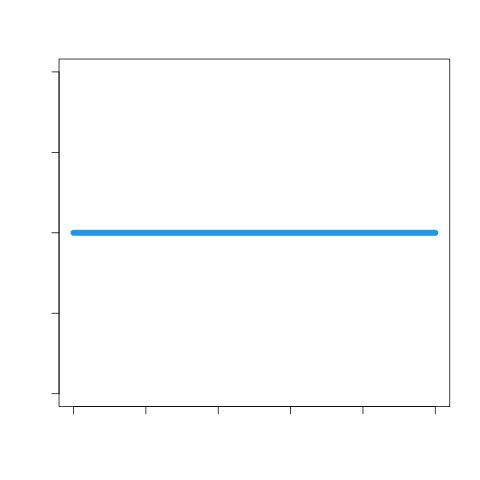
\includegraphics[width=.18\textwidth]{\fignet/FigMotifsBEDD-dist-h10} \end{tabular} &
    \begin{tabular}{c} 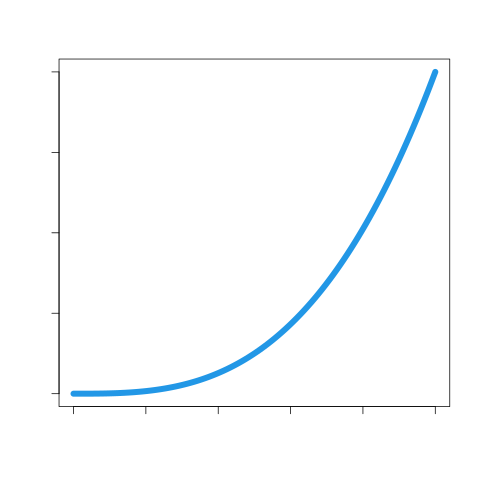
\includegraphics[width=.18\textwidth]{\fignet/FigMotifsBEDD-dist-h40} \end{tabular} \\
    \begin{tabular}{c} $g_0(u) =$ \end{tabular} &
    \begin{tabular}{c} 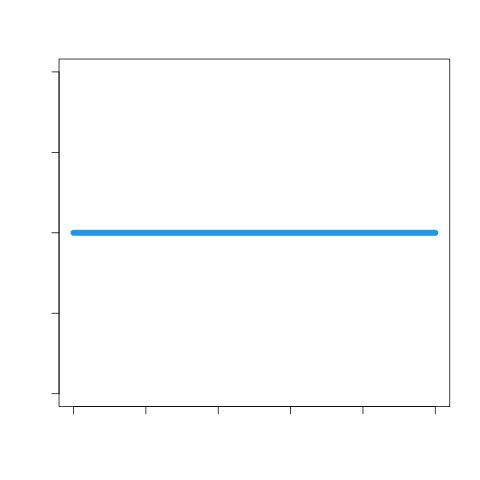
\includegraphics[width=.18\textwidth]{\fignet/FigMotifsBEDD-dist-g10} \end{tabular} &
    \begin{tabular}{c} 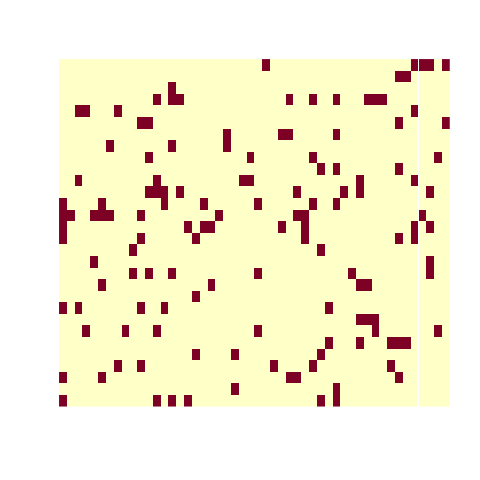
\includegraphics[width=.18\textwidth]{\fignet/FigMotifsBEDD-adj-g10-h10} \end{tabular} &
    \begin{tabular}{c} 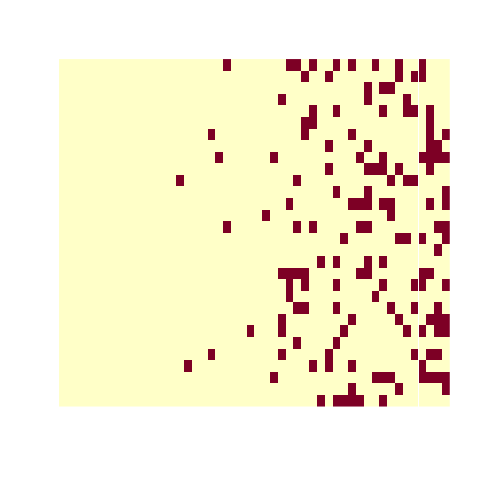
\includegraphics[width=.18\textwidth]{\fignet/FigMotifsBEDD-adj-g10-h40} \end{tabular} \\
    \begin{tabular}{c} $g(u) =$ \end{tabular} &
    \begin{tabular}{c} 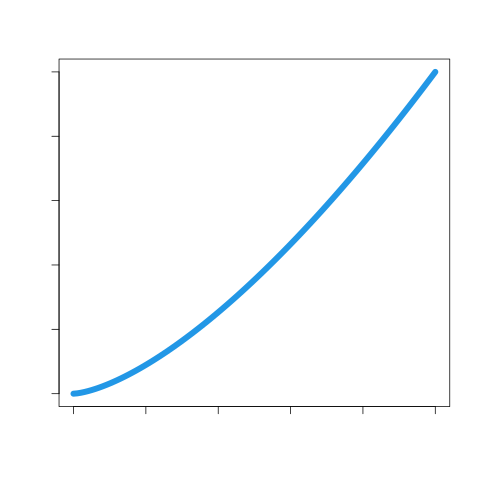
\includegraphics[width=.18\textwidth]{\fignet/FigMotifsBEDD-dist-g25} \end{tabular} &
    \begin{tabular}{c} 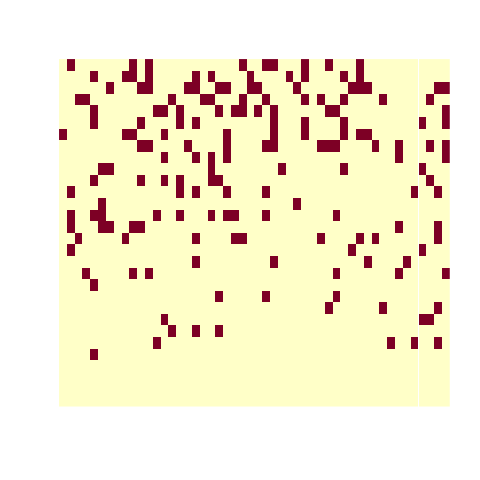
\includegraphics[width=.18\textwidth]{\fignet/FigMotifsBEDD-adj-g25-h10} \end{tabular} &
    \begin{tabular}{c} 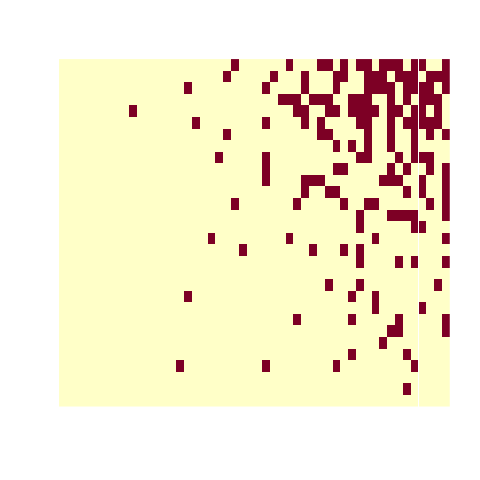
\includegraphics[width=.18\textwidth]{\fignet/FigMotifsBEDD-adj-g25-h40} \end{tabular} \\
  \end{tabular}
  
%   \bigskip 
%   \paragraph{Sufficient statistics} to fit BEDD: stars (top, bottom, single edge) frequencies

}

\backupend

%==================================================================
%==================================================================
\end{document}
%==================================================================
%==================================================================

\begin{tabular}{ll}
  \begin{tabular}{p{.45\textwidth}}
  \end{tabular}
  &
  \begin{tabular}{p{.45\textwidth}}
  \end{tabular} 
\end{tabular}

